\documentclass[twocolumn]{article}   % list options between brackets
\usepackage{}              % list packages between braces

\usepackage{graphicx}
\usepackage[dvipsnames]{xcolor} % Package used for coloured text
\usepackage{csvsimple,longtable}
\usepackage{amssymb}
\usepackage{amsmath}
\usepackage{etoolbox}
\usepackage{tikz} % To generate the plot from csv
\usepackage{pgfplots}
\usepackage{siunitx}
\usepackage{soul}
\usepackage[section]{placeins}
%\usepackage[margin={.75in,.75in}]{geometry}
\usepackage[a4paper,margin=1cm,footskip=.5cm]{geometry}

\makeatletter % change only the display of \thepage, but not \thepage itself:
\patchcmd{\ps@plain}{\thepage}{\textcolor{orange}{\thepage}}{}{}
\makeatother
\pagestyle{plain}

% for graphs
  \pgfplotsset{compat=newest} % Allows to place the legend below plot
  \usepgfplotslibrary{units} % Allows to enter the units nicely

  \sisetup{
    round-mode          = places,
    round-precision     = 2,
  }

\begin{document}

% Title Page

  \title{Python project report \\~\\  \small{an Introduction to Computer Programming coursework}}    % type title between braces

  \author{\color{orange} {Dan Gorringe} \\ \small{\color{orange}dg17129@my.bristol.ac.uk}}        % type author(s) between braces
  %\date{6th February, 2017}    % type date between braces
  \maketitle

% Contents Page
%\tableofcontents{}

%Introduction
\section{Introduction}

For an Introduction to Computer program we are set an open ended python project for 60\% of the unit:
  \begin{quote}
    "The objective of Assignment 2 is to write an original Python program that shows off
your Python programming skills and some of your creative flair"
  \end{quote}

After having completed my previous scratch project: It dawned on me that I hadn't thought about the examiner, how to get the highest score for my project. I realised that the marker probably doesn't like stupid side scrolling games, so "what do they like?" is what I asked myself. I knew they must like allocating marks, as they do it so much, and like that: it came to me! A marking Simulator! What more could somebody who has to mark 186 other projects want to do more than have to mark more? In hindsight they may prefer to read about the pitfalls and agony of a smart-arse.

\section{How to run the game}
To run make sure you have python3. You will also need the following modules: random, tkinter, PIL, math, functools. Then all the files to run are found within the \texttt{src} directory.

\section{How to play the game}
To play the game simply load up game.py, then choose wether you would like to mark some \st{pretentious} art or \st{stupidly easy} maths. You then mark each 'persons' piece of work, one at a time. Once you've marked all of them you follow the windows, seeing how badly you've done before being taken back to the original window.

\section{Design ethos}
To ensure I could backup my project and not lose whilst I travelled around over the festive season I created an private repository on Github for my python project. I keep all the python within the \texttt{src} directory, and all the tex for this report within the \texttt{report} directory.
It was my aim to have one 'guiding' python file, to tell the 'story' of the game. Hence I created several classes which I kept in seperate files and import to the main \texttt{game.py}. I tried to keep to camelCase within this project.
  \subsection{and associated pitfalls}
  Due to almost everything being within their own class I frequently ran into trouble by not having self littered around the place. I also found it difficult to be able to access data that I wanted from particular instances of classes.

\section{Tkinter}
To make all the GUI elements I used TKinter\cite{TKinter}, which comes preinstalled with python. I had some issues when using their IntVars and StringVars, I believe this was due to a cocktail of both not knowing you need to use \texttt{.set} and \texttt{.get()} to change the variable and with some odd happenings with \texttt{.pack()} always returning 0, thus negating the intended \texttt{.get()} functionality.
  \subsection{command issues}
  I Also had problems when trying to set the command of buttons, TKinter alone does not seem to like giving a functino with argument. So I had to use some functools wizard (the syntax of which I found online) to pass an argument so that I could mark a specific artifact. I also had to use lambda in another scenario and in another did not need to use it at all as was running a function inside a class with no argument.

\section{Criteria}
The simplest class that I created, hence it has not changed since December. They mearly contain a string of their name, a brief description, wether they are critical and what their maximum is. In the beginning I had intentions to deeply imbed plagarism, to force the player to root out all plagarists and award no marks. However as time slipped away so did my intentions of implementing, but you can still find variables for plagarism ready to be implemented. I instantiate these criteria at the start of the \texttt{game.py} file

\section{Artifact}
The Artifacts are the individual 'pieces of work'. They include the question that they're answering, their 'answer', who 'they' are, the list of criteria to be marked against and what their values for this are (what marks should be alocated).
Initally the answer was used just for the maths question, when I branched out to include the picture question too I changed the answer to be the name of an image to use to dispaly on the atifact window. Therefore I can easily add in any type of question to all the existing infastructure as long as I can generate an image to represent it.
  \subsection{and associated pitfalls}
  I came across issues when I was trying to insert a picture into the tkinter windows, This stumpted me for a while, however I finally came to the realisation that It was because of the lack of self (.self). This caused much panic, as for a time too long, too near the deadline I was unable to present any articles to be marked. I also have to use some funny Tkinter add on to allow images.
  \subsection{Names}
  I also create psuedo random names for all artifacts. I made seperate text files for first names and surnames: I made sure to include all the members of S Club 7 and lecturers. I load these into arrays and randomly assign one of each to create the author. I use this same technique to randomise the person for which you owe losing 200 points if you incorrectly mark a maths artifact.

\section{Questions}
Each artifact has a question that it is for. The Question class is responsible for generating images. To work out how to produce these images I had to google tutorials, however I found lots of these missed out lots of details, so instead eneded up using the documentation for PIL\cite{PIL}. I came across funny nuances with the python image libary, one of which that it only likes gifs, so made sure to only save as gifs instead of the JPEGs that I did originally.
  \subsection{Basic Maths}
  I started with a basic algebra question. To initialise you give it a random integer and an integer of the answer.
  \subsection{Sun picture}
  I then made another assignment to be marked, more artsy this time: to put my criteria classes to good use. I used PIL to create image. I created a list of different RGB tuples, all semi-sun-ish. I also created several sub lists: topTierColours, avantGardeColours, shittyColours and pastelColours. Where the colours used in the image comes from depends on how 'onTopic' the artifact is deemed to be. The complexity effects how intricate the image is, how many ellipses are placed. The onTopic factor also effects how circular the ellipses are, as everyone knows the sun is round.

\section{Progressbar}
I had lots of trouble with the progress bar, initally I tried using an IntVar however I gave up and instead kept resetting the config of the actual progress bar instead.

\section{Backup Graphing}
As I only had a few days left when I came across the spinbox issues I started to majorly panic. So I decided to try make a 'backup' project. I made a program which plotted functions on a terminal using unicode full blocks, and using the same kind of technique produced a bitcoin tracker. In my panic I overwrote the bitcoin tracker, though some video of it remains in circulation, but I managed to get the graphing script to work again. There is a backup folder which contains this graphing file, which should show the cos wave on a terminal, to the currect size. This nearly then came in useful whilst trying to do the progress window for a round, however just led to more time loss. I had a series of labels, and I could iterate down them to try produce a graph, however tkinter has it out for me and has different spacing between characters so instead of waste more time, this idea went into the bin.

\begin{figure}
  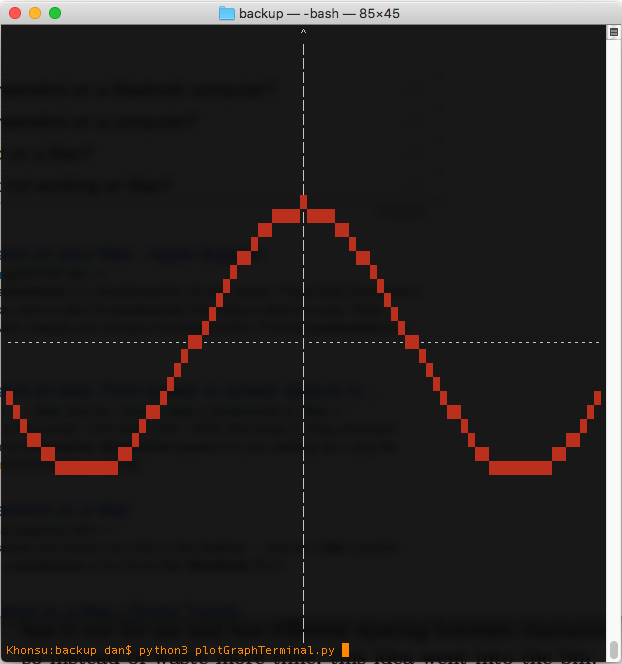
\includegraphics[width=0.5\textwidth]{graphScreenshot}
  \caption{A panicked attempt to plot of cos(x)}
\end{figure}

\section{Menu}
After having got both question rounds running I quickly realised that I needed a way to control these. I decided upon yet another class, self entitled. However since this is the controlling element I though that it deserved to be within the main \texttt{game.py} file. The display function within merely opens a window, with a label which can be changed to dispaly the score and buttons for both question types. I have a function for each question type, to create and run each. Both buttons end with calling a \texttt{playingState} function, this is intended to be entered whilst the player is otherwise occupied marking work, it unpacks the buttons to start new rounds and replaces with a continue. When the continue button is pressed a function is run to return the score earnt over the round played, these score is added to the current score and the label updated, with the buttons to create new rounds reappearing, to create endless \st{fun} gameplay.

\section{Theme}
I had originally planned to make the game very much like papers please\, to use graphics to dispaly the information. However as time got behind me I realised this was not going to be feesible and instead opted for TKinter.

\section{Conclusion}
I think that I hugely benefited from having a robust infastructure. It was incredibly easy to add in the second question type and would be easier now to add more questions if I had time to think up and implement new questions and their respective randomly generated images. And that was the crux of this project, I thought I could do way more with the time and simply started running out of time. I would have loved to have a bigger selection of questions and to have it all within it's own nice graphics. In the future I'd make sure to restrict myself to using fewer external libaries and lots of time was lost trying to get these to work how I wanted them to. I will also not set such a high bar to begin with.

\begin{thebibliography}{9}

  \bibitem{PIL}
  Pillow - Python module
  \\\texttt{https://python-pillow.org/}

  \bibitem{TKinter}
  TKinter - Python module
  \\\texttt{https://docs.python.org/2/library/tkinter.html}

  \bibitem{Papers}
  Papers, please - Wikipedia
  \\\texttt{www.youtube.com/watch?v=\_QP5X6fcukM}

\end{thebibliography}


%\begin{figure}[pb!]
%  \includegraphics[width=3in]{./Images/MahogonyDoor.jpg}
%\end{figure}


\end{document}
